\documentclass[aspectratio=169,11pt]{ctexbeamer}

% ── Theme ──────────────────────────────────────────────────────────
\usetheme{Madrid}
\usecolortheme{whale}
\setbeamertemplate{navigation symbols}{}
\setbeamertemplate{footline}[frame number]
\setbeamerfont{frametitle}{size=\large,series=\bfseries}

% ── Packages ───────────────────────────────────────────────────────
\usepackage{amsmath,amssymb}
\usepackage{graphicx}
\usepackage{booktabs}
\usepackage{tikz}
\usetikzlibrary{arrows.meta,positioning,shapes.geometric,shapes.misc,calc,decorations.pathreplacing}
\usepackage{xcolor}
\usepackage{appendixnumberbeamer}

% ── Colors ─────────────────────────────────────────────────────────
\definecolor{cA}{RGB}{220,80,60}      % Scheme A — red
\definecolor{cC}{RGB}{50,140,70}      % Scheme C — green
\definecolor{cOracle}{RGB}{40,100,180}% Oracle — blue
\definecolor{cHighlight}{RGB}{230,160,30} % highlight gold
\definecolor{cBg}{RGB}{245,245,250}
\definecolor{cDarkBg}{RGB}{30,55,90}

% ── Math shortcuts ─────────────────────────────────────────────────
\newcommand{\E}{\mathbb{E}}
\newcommand{\R}{\mathbb{R}}
\newcommand{\V}{\mathbb{V}}
\newcommand{\wbar}{\bar{w}}
\newcommand{\what}{\hat{w}}
\newcommand{\wstar}{w^*}
\DeclareMathOperator*{\argmax}{arg\,max}

% ── Meta ───────────────────────────────────────────────────────────
\title[FedProTrack]{先聚类，再训练\\[4pt]
  \normalsize 基于数据指纹的联邦学习概念发现\\
  ——面向周期性概念漂移场景}
\author{}
\date{2026年4月}
\institute{}

% ===================================================================
\begin{document}

% -------------------------------------------------------------------
\begin{frame}[plain]
\titlepage
\end{frame}

% -------------------------------------------------------------------
\begin{frame}{目录}
\tableofcontents
\end{frame}

% ===================================================================
\section{背景与动机}
% ===================================================================

% -------------------------------------------------------------------
\begin{frame}{问题设定：概念漂移下的联邦学习}

\begin{columns}[T]
\begin{column}{0.55\textwidth}
\begin{itemize}
  \item $K$ 个客户端，$T$ 轮通信，$C$ 个隐含\textbf{概念}
  \item 每轮中，客户端 $k$ 从概念 $c(k,t)\in[C]$ 的分布采样数据
  \item 概念会\textbf{周期性复现}：客户端访问概念 $b$ 后可能回到概念 $a$
  \item 服务器无法看到原始数据——只能通过聚合信号间接推断
\end{itemize}

\vspace{6pt}
\textbf{目标}：推断隐含概念身份 $\to$ 分组客户端 $\to$ 按概念联邦聚合

\vspace{6pt}
\textcolor{cOracle}{\textbf{Oracle}}（性能上界）：每轮已知真实 $c(k,t)$
\end{column}

\begin{column}{0.42\textwidth}
\centering
\begin{tikzpicture}[
    client/.style={circle,draw,minimum size=7mm,font=\small},
    concept/.style={rounded rectangle,draw,thick,minimum height=7mm,font=\small},
    >=Stealth, scale=0.85, transform shape
  ]
  % Concepts
  \node[concept,fill=red!15]   (cA) at (0,2.5) {概念 A};
  \node[concept,fill=blue!15]  (cB) at (2.8,2.5) {概念 B};
  % Clients
  \foreach \i/\x in {1/0, 2/1, 3/2, 4/3} {
    \node[client,fill=gray!10] (k\i) at (\x, 0) {$k_{\i}$};
  }
  % Assignments (round t)
  \draw[->,thick,red!60]  (cA) -- (k1);
  \draw[->,thick,red!60]  (cA) -- (k2);
  \draw[->,thick,blue!60] (cB) -- (k3);
  \draw[->,thick,blue!60] (cB) -- (k4);
  % Server
  \node[rectangle,draw,fill=cDarkBg,text=white,minimum width=30mm,minimum height=7mm,font=\small\bfseries] (srv) at (1.5,-1.5) {服务器};
  \foreach \i in {1,...,4} {
    \draw[<->,gray,dashed] (srv) -- (k\i);
  }
  % Label
  \node[font=\scriptsize,gray] at (1.5,3.3) {第 $t$ 轮：隐含概念分配};
\end{tikzpicture}
\end{column}
\end{columns}
\end{frame}

% -------------------------------------------------------------------
\begin{frame}{核心设计选择：何时聚类？}
\centering
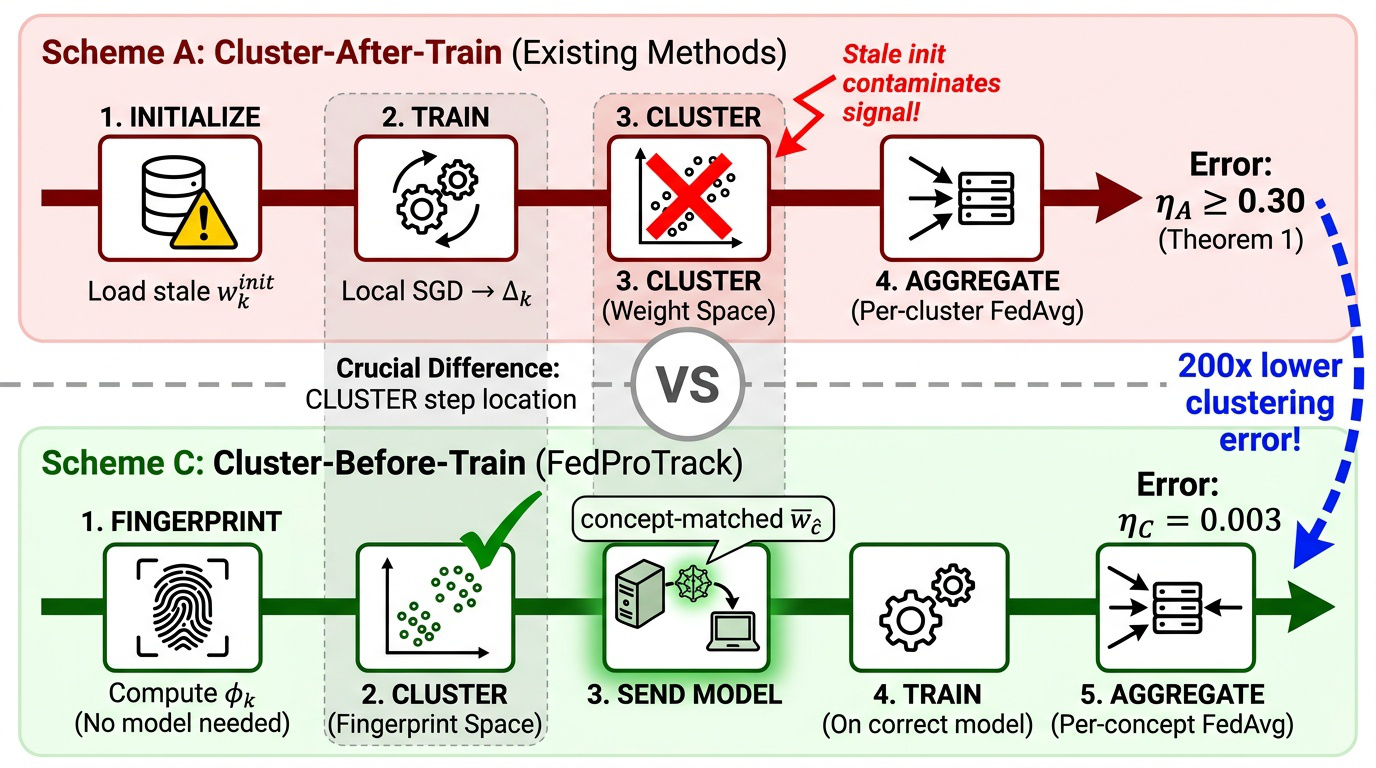
\includegraphics[width=0.82\textwidth]{figures/paperbanana/scheme_comparison_candidate_0.png}

\vspace{1pt}
{\scriptsize
\textbf{定理 1}：$\eta_A \geq \eta_A^{(\mathrm{clean})} + \kappa \cdot \V(w^{(\mathrm{init})})$ \quad
$\Rightarrow$ \textcolor{cA}{方案 A：$\eta \geq 0.30$} \quad vs \quad \textcolor{cC}{方案 C：$\eta = 0.003$}
}
\end{frame}

% ===================================================================
\section{理论基础}
% ===================================================================

% -------------------------------------------------------------------
\begin{frame}{概念级聚合何时有效？}
\centering
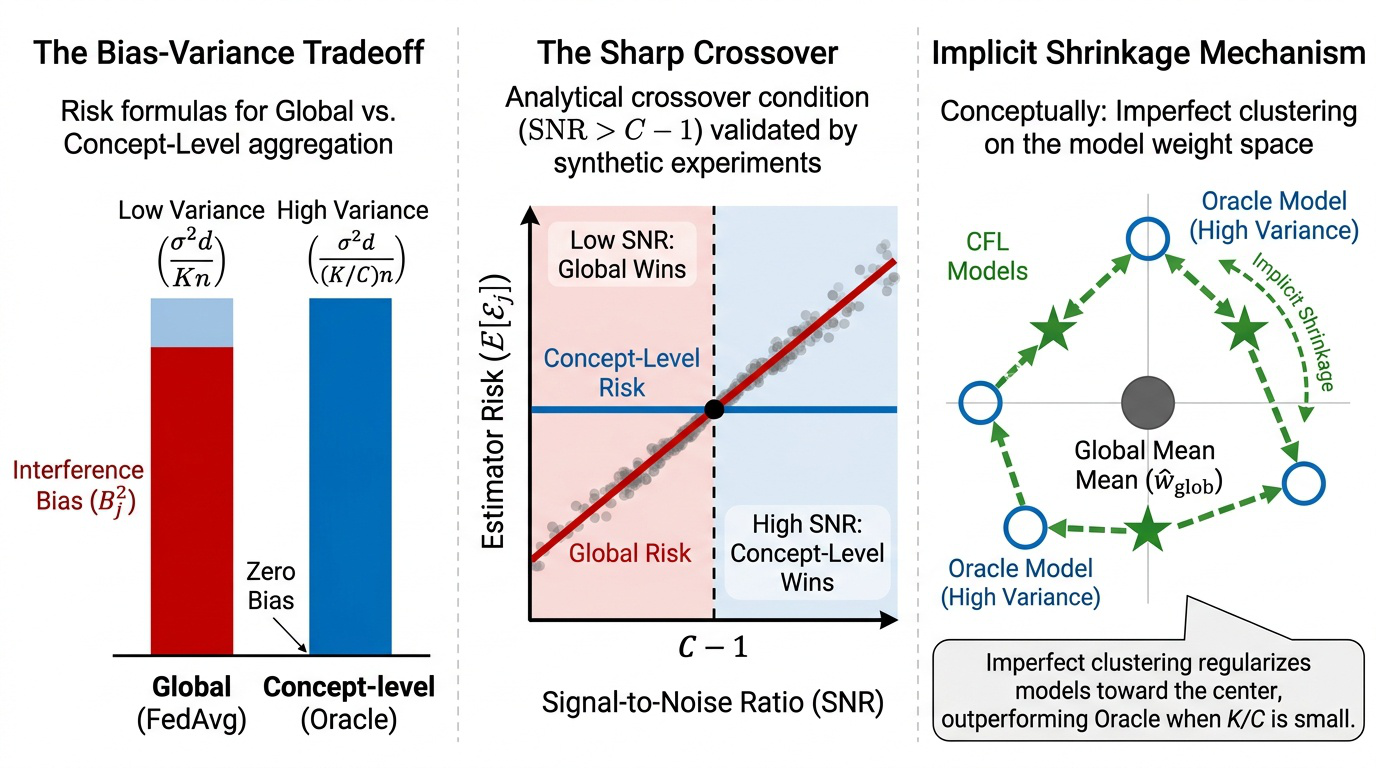
\includegraphics[width=0.78\textwidth]{figures/paperbanana/research_question_candidate_2.png}

\vspace{1pt}
{\scriptsize
\textbf{左}：偏差-方差权衡 \quad
\textbf{中}：在 $\mathrm{SNR} = C{-}1$ 处的尖锐交叉点 \quad
\textbf{右}：不完美聚类 $=$ 隐式收缩
}
\end{frame}

% -------------------------------------------------------------------
\begin{frame}{现有方法：方案 A（先训练后聚类）}

\textbf{几乎所有}聚类联邦学习方法都遵循同一协议：

\vspace{8pt}
\begin{tikzpicture}[
    box/.style={rectangle,draw,rounded corners=3pt,minimum height=10mm,minimum width=22mm,font=\small,align=center},
    >=Stealth, node distance=8mm
  ]
  \node[box,fill=gray!10] (init) {加载上轮\\模型 $w_k^{(\mathrm{init})}$};
  \node[box,fill=orange!15,right=of init] (train) {本地\\训练};
  \node[box,fill=cA!15,right=of train] (cluster) {对 $\{\Delta_k\}$\\聚类};
  \node[box,fill=blue!10,right=of cluster] (agg) {分组\\FedAvg};
  \draw[->,thick] (init) -- (train);
  \draw[->,thick] (train) -- (cluster);
  \draw[->,thick] (cluster) -- (agg);
  \node[font=\scriptsize,gray,above=1mm of init] {步骤 1};
  \node[font=\scriptsize,gray,above=1mm of train] {步骤 2};
  \node[font=\scriptsize,gray,above=1mm of cluster] {步骤 3};
  \node[font=\scriptsize,gray,above=1mm of agg] {步骤 4};
\end{tikzpicture}

\vspace{10pt}
\textbf{典型方法}：IFCA、CFL、FedEM、FedRC、FedGWC、基于梯度的划分\ldots

\vspace{10pt}
\begin{alertblock}{隐含假设}
权重更新 $\Delta_k$ 能忠实反映客户端的\emph{当前}概念身份。
\end{alertblock}

\vspace{4pt}
\textcolor{cA}{\textbf{但在概念复现场景下，这一假设不成立。}}
\end{frame}

% -------------------------------------------------------------------
\begin{frame}{陈旧初始化问题}

当客户端从概念 $a$ 切换到概念 $b$ 时，它加载的是上次在 $a$ 上训练的模型：

\begin{equation*}
\Delta_k = \underbrace{-\alpha \nabla L_b(\wbar_b)}_{\text{真实概念-}b\text{ 信号}}
          + \underbrace{\alpha H_k \bigl(w_k^{(\mathrm{init})} - \wbar_b^{(t-1)}\bigr)}_{\textcolor{cA}{\text{陈旧初始化污染}}}
          + O(\|\cdot\|^2)
\end{equation*}

\begin{itemize}
  \item 污染项与概念 $b$ \textbf{完全无关}
  \item 其大小正比于 $\|w_k^{(\mathrm{init})} - \wbar_b\|$——即"初始化失配"
  \item 任何在 $\Delta_k$ 上做聚类的算法都会被\textbf{结构性误导}
\end{itemize}

\vspace{4pt}
\centering
\textcolor{cA}{\textbf{$\Rightarrow$ 这不是算法问题——而是协议结构问题。}}
\end{frame}

% -------------------------------------------------------------------
\begin{frame}{定理：陈旧初始化放大效应}

\begin{theorem}[主定理——无条件成立]
在标准正则性条件下（$L$-光滑，$\mu$-强凸）：
\begin{equation*}
\boxed{\eta_A \;\geq\; \eta_A^{(\mathrm{clean})} \;+\; \kappa \cdot \V(w^{(\mathrm{init})})}
\end{equation*}
其中 $\V(w^{(\mathrm{init})}) > 0$ \textbf{只要概念存在复现}。
\end{theorem}

\vspace{6pt}
三个关键推论：
\begin{enumerate}
  \item \textbf{无条件}：仅需标准假设，无需额外条件
  \item $\V(w^{(\mathrm{init})}) > 0$ 在概念复现下是\textbf{结构性}的——\textbf{无法消除}
  \item 方案 A 框架内的任何算法改进都无法缩小这一差距
\end{enumerate}

\vspace{6pt}
\textbf{从聚类误差到多余风险}（推论 1）：\\[2pt]
结合隐式收缩刻画，多余风险差距\\
$\geq (\eta_A - \eta_C) \cdot \frac{C}{C-1} \cdot \bar{B}^2 > 0$
\end{frame}

% -------------------------------------------------------------------
\begin{frame}{实验证据：所有方案 A 方法均 $\eta \geq 0.30$}

\begin{columns}[T]
\begin{column}{0.48\textwidth}
\centering
\begin{tikzpicture}[scale=0.85, transform shape]
  % Bar chart: clustering error
  \draw[->] (0,0) -- (0,4.5) node[above,font=\small] {$\eta$（聚类误差）};
  \draw[->] (0,0) -- (5.5,0);
  % bars
  \fill[cC!70] (0.3,0) rectangle (1.1, 0.12);  % FPT
  \fill[cA!50] (1.5,0) rectangle (2.3, 3.04);  % CFL
  \fill[cA!50] (2.7,0) rectangle (3.5, 3.20);  % IFCA
  \fill[cA!50] (3.9,0) rectangle (4.7, 3.84);  % FedEM
  % labels
  \node[font=\scriptsize,rotate=45,anchor=east] at (0.7,-0.1) {FPT};
  \node[font=\scriptsize,rotate=45,anchor=east] at (1.9,-0.1) {CFL};
  \node[font=\scriptsize,rotate=45,anchor=east] at (3.1,-0.1) {IFCA};
  \node[font=\scriptsize,rotate=45,anchor=east] at (4.3,-0.1) {FedEM};
  % values
  \node[font=\scriptsize,cC] at (0.7, 0.45) {\textbf{0.003}};
  \node[font=\scriptsize,cA] at (1.9, 3.35) {0.38};
  \node[font=\scriptsize,cA] at (3.1, 3.55) {0.40};
  \node[font=\scriptsize,cA] at (4.3, 4.15) {0.48};
  % threshold line
  \draw[dashed,thick,cA] (0,2.4) -- (5.3,2.4) node[right,font=\scriptsize] {$\eta = 0.30$};
  % scale
  \foreach \y/\v in {0/0, 0.8/0.10, 1.6/0.20, 2.4/0.30, 3.2/0.40, 4.0/0.50} {
    \draw (0,\y) -- (-0.1,\y) node[left,font=\tiny] {\v};
  }
\end{tikzpicture}
\end{column}

\begin{column}{0.50\textwidth}
\begin{itemize}
  \item 在 CIFAR-100 上，\textbf{所有}方案 A 方法：$\eta \geq 0.38$
  \item FPT 达到 $\eta = 0.003$——\textbf{低两个数量级}
  \item 该差距是\emph{结构性}的，非算法差异
\end{itemize}

\vspace{8pt}
\textbf{即使使用 Oracle 初始化}（消除 $\V$）：\\
$\eta_A^{(\mathrm{clean})} = 0.40$ vs $\eta_C = 0.002$

\vspace{6pt}
$\Rightarrow$ 指纹具有内在的 $d/L$ 信噪比优势\\
\quad （引理 2：$d=128$，$L=10$ $\Rightarrow$ $12.8\times$）
\end{column}
\end{columns}
\end{frame}

% ===================================================================
\section{方法：FedProTrack}
% ===================================================================

% -------------------------------------------------------------------
\begin{frame}{FedProTrack：总览}
\centering
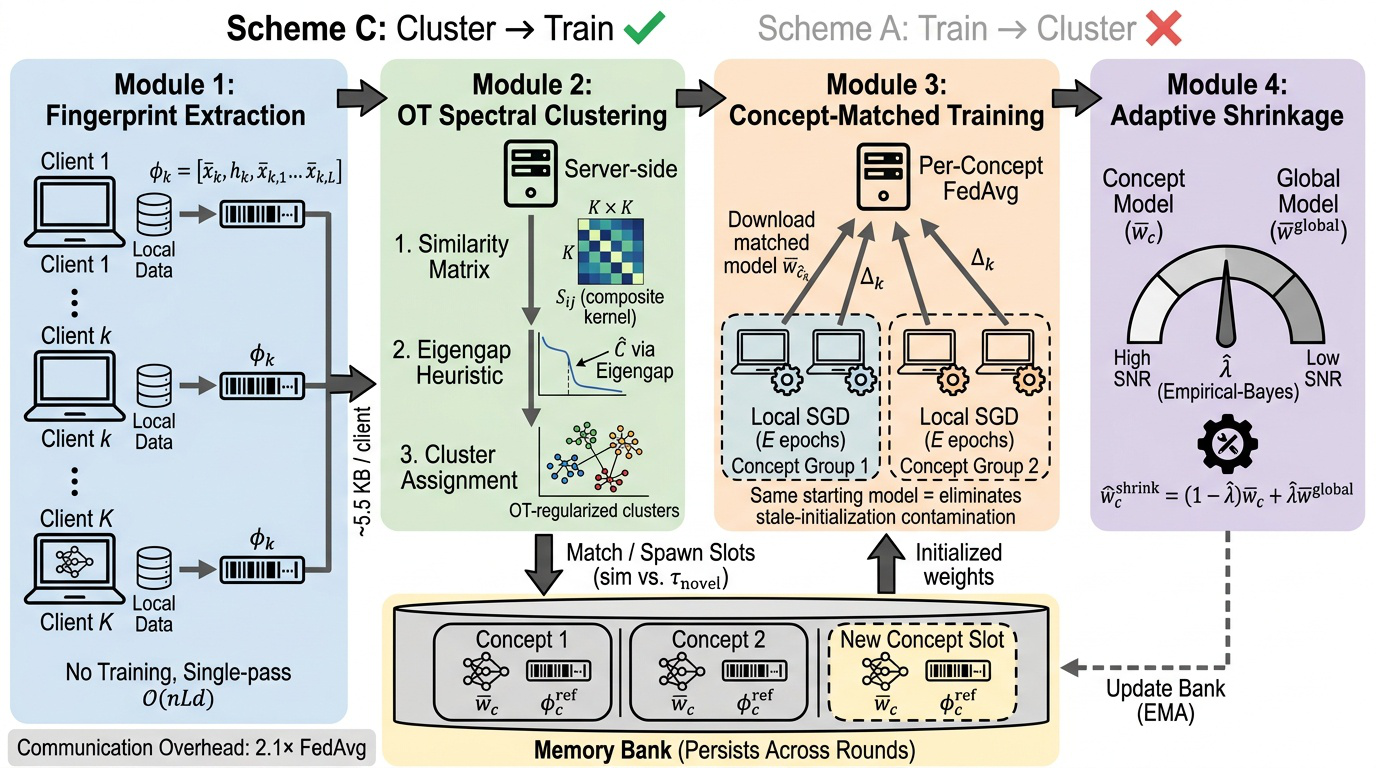
\includegraphics[width=0.78\textwidth]{figures/paperbanana/pipeline_v2_candidate_1.png}

\vspace{1pt}
{\scriptsize
\textbf{方案 C}：指纹提取 $\to$ OT 谱聚类 $\to$ 概念匹配训练 $\to$ 自适应收缩（$2.1\times$ FedAvg 通信量）
}
\end{frame}

% -------------------------------------------------------------------
\begin{frame}{模块 1：指纹提取}

\small
每个客户端\textbf{无需模型训练}即可计算数据指纹：
\vspace{-4pt}
$$\phi_k = \bigl[\underbrace{\bar{x}_k}_{\text{全局均值}},\;\;
         \underbrace{h_k}_{\text{标签分布}},\;\;
         \underbrace{\bar{x}_{k,1},\;\ldots,\;\bar{x}_{k,L}}_{\text{类条件均值}}\bigr]$$

\vspace{-6pt}
\begin{columns}[T]
\begin{column}{0.50\textwidth}
\textbf{为什么这样设计？}
\begin{itemize}\setlength\itemsep{0pt}
  \item 类条件均值 $=$ 概念身份的\textbf{充分统计量}
  \item 单次扫描 $O(nLd)$，无需梯度计算
  \item $d{=}128$，$L{=}10$ $\Rightarrow$ 每客户端仅 \textbf{5.5 KB}
\end{itemize}
\end{column}

\begin{column}{0.48\textwidth}
\textbf{信噪比优势（引理 2）：}
\vspace{-6pt}
$$\frac{\mathrm{SNR}_{\mathrm{fp}}}{\mathrm{SNR}_{\mathrm{wt}}} = \frac{d}{L} = \frac{128}{10} = 12.8\times$$
\vspace{-6pt}

指纹以\emph{一阶}矩编码概念信号；权重则将其埋入\emph{二次}形式（$X^\top X$）中。
\end{column}
\end{columns}
\end{frame}

% -------------------------------------------------------------------
\begin{frame}{模块 2：OT 谱聚类——步骤 1：相似度矩阵}

给定 $K$ 个指纹 $\{\phi_1, \ldots, \phi_K\}$，服务器计算：

\begin{equation*}
S_{ij} = \underbrace{0.25 \cdot \mathrm{sim}_{\mathrm{feat}}(\phi_i, \phi_j)}_{\text{全局均值高斯核}}
       + \underbrace{0.30 \cdot \mathrm{sim}_{\mathrm{label}}(h_i, h_j)}_{\text{标签直方图余弦相似}}
       + \underbrace{0.45 \cdot \mathrm{sim}_{\mathrm{cc}}(\phi_i, \phi_j)}_{\text{类条件高斯核}}
\end{equation*}

\vspace{4pt}
\begin{itemize}\setlength\itemsep{2pt}
  \item 权重在留出的合成数据上固定，\textbf{不在评估数据上调优}
  \item $\mathrm{sim}_{\mathrm{cc}}$ 权重最大：类条件结构携带最多概念信号
  \item \textbf{鲁棒性}：4 种权重配置下精度变化 $\leq 0.2$pp
\end{itemize}

\vspace{4pt}
\textbf{理论联系}：对于共享协方差的高斯类分布，类条件均值的欧氏距离 $\approx$ \textbf{Wasserstein-2}：
$\;W_2^2(P_a, P_b) = \sum_c w_c \|\mu_a^{(c)} - \mu_b^{(c)}\|^2$
\end{frame}

% -------------------------------------------------------------------
\begin{frame}{模块 2：OT 谱聚类——步骤 2：特征间隙}

通过归一化拉普拉斯矩阵\textbf{自动确定概念数量}：

\begin{columns}[T]
\begin{column}{0.52\textwidth}
\begin{enumerate}
  \item 构造 $L_{\mathrm{sym}} = I - D^{-1/2}SD^{-1/2}$
  \item 计算特征值 $\lambda_1 \leq \lambda_2 \leq \cdots \leq \lambda_K$
  \item 找到最大间隙：
    $$\hat{C} = \argmax_{c \in [2, K/2]} (\lambda_{c+1} - \lambda_c)$$
\end{enumerate}

\vspace{6pt}
\textbf{直觉}：$C$ 个分离良好的簇 $\Rightarrow$ $C$ 个特征值 $\approx 0$，然后出现\textbf{跳跃}

\vspace{6pt}
\textcolor{cC}{\textbf{结果}}：特征间隙在 $>$95\% 的轮次中正确恢复 $\hat{C}{=}4$。固定 $\hat{C}{=}C$ 仅损失 0.6pp。
\end{column}

\begin{column}{0.45\textwidth}
\centering
\begin{tikzpicture}[scale=0.82, transform shape]
  % Axes
  \draw[->] (0,0) -- (6.5,0) node[right,font=\small] {序号 $i$};
  \draw[->] (0,0) -- (0,4.5) node[above,font=\small] {$\lambda_i$};
  % Eigenvalues
  \filldraw[cC] (0.5, 0.1) circle (3pt);
  \filldraw[cC] (1.2, 0.15) circle (3pt);
  \filldraw[cC] (1.9, 0.25) circle (3pt);
  \filldraw[cC] (2.6, 0.35) circle (3pt);
  % Gap
  \draw[<->,thick,cHighlight] (3.0, 0.35) -- (3.0, 2.8)
    node[midway,right,font=\small\bfseries,text=cHighlight] {eigengap!};
  % Noise plateau
  \filldraw[cA] (3.3, 2.8) circle (3pt);
  \filldraw[cA] (4.0, 3.0) circle (3pt);
  \filldraw[cA] (4.7, 3.15) circle (3pt);
  \filldraw[cA] (5.4, 3.3) circle (3pt);
  % Labels
  \draw[decorate,decoration={brace,amplitude=4pt},thick,cC]
    (0.3,-0.3) -- (2.8,-0.3) node[midway,below=4pt,font=\small,cC] {结构特征值（$\hat{C}{=}4$）};
  \draw[decorate,decoration={brace,amplitude=4pt},thick,cA]
    (3.1,-0.3) -- (5.6,-0.3) node[midway,below=4pt,font=\small,cA] {噪声平台};
\end{tikzpicture}
\end{column}
\end{columns}
\end{frame}

% -------------------------------------------------------------------
\begin{frame}{模块 2：OT 谱聚类——步骤 3：OT 正则化分配}
\small
\begin{columns}[T]
\begin{column}{0.55\textwidth}
\textbf{标准谱聚类}：取前 $\hat{C}$ 个特征向量 $\to$ 行归一化 $\to$ $k$-means。

\vspace{4pt}
\textbf{问题}：$k$-means 可能产生空/极小簇——1 个客户端的组没有聚合收益。

\vspace{4pt}
\textbf{OT 正则化}替代 $k$-means：
\vspace{-4pt}
$$\min_{\pi} \sum_{i,c} \pi_{ic} \|v_i - \mu_c\|^2$$
\vspace{-10pt}
\begin{align*}
\text{s.t.}\;\; \sum_c \pi_{ic} &= 1 \;\;\forall i \\
\sum_i \pi_{ic} &\geq \lfloor K/(2\hat{C}) \rfloor \;\;\forall c \;\;\textcolor{cC}{\text{（最小簇大小）}}
\end{align*}
\end{column}

\begin{column}{0.42\textwidth}
\centering
\begin{tikzpicture}[scale=0.55, transform shape]
  % k-means failure
  \node[font=\small\bfseries] at (2.5, 5.2) {标准 $k$-means};
  \fill[red!10,rounded corners] (0,2.5) rectangle (5,5);
  \filldraw[cA!70] (1,4) circle (3pt);
  \filldraw[cA!70] (1.3,3.8) circle (3pt);
  \filldraw[cA!70] (0.8,3.5) circle (3pt);
  \filldraw[cA!70] (1.5,4.2) circle (3pt);
  \filldraw[cOracle!70] (3.5,4) circle (3pt);
  \filldraw[cOracle!70] (3.8,3.6) circle (3pt);
  \filldraw[cOracle!70] (3.3,3.4) circle (3pt);
  \filldraw[cHighlight] (4.5,2.8) circle (3pt);
  \node[font=\tiny,right] at (4.7,2.8) {孤立！};
  % OT fix
  \node[font=\small\bfseries,cC] at (2.5, 2.2) {+ OT 约束};
  \fill[green!5,rounded corners] (0,0) rectangle (5,2);
  \filldraw[cA!70] (1,1.2) circle (3pt);
  \filldraw[cA!70] (1.3,1) circle (3pt);
  \filldraw[cA!70] (0.8,0.7) circle (3pt);
  \filldraw[cA!70] (1.5,1.4) circle (3pt);
  \filldraw[cOracle!70] (3.5,1.2) circle (3pt);
  \filldraw[cOracle!70] (3.8,0.8) circle (3pt);
  \filldraw[cOracle!70] (3.3,0.6) circle (3pt);
  \filldraw[cOracle!70] (3.6,1.5) circle (3pt);
  \filldraw[cOracle!70] (4.3,1) circle (3pt);
  \node[font=\tiny,cC] at (2.5,-0.3) {最小簇 $\geq \lfloor K/(2\hat{C})\rfloor$};
\end{tikzpicture}
\end{column}
\end{columns}
\end{frame}

% -------------------------------------------------------------------
\begin{frame}{模块 3：记忆库与概念匹配}
\small
\begin{columns}[T]
\begin{column}{0.56\textwidth}
记忆库 $\mathcal{M} = \{(\wbar_c, \phi_c^{\mathrm{ref}})\}$ 存储每个概念的模型和参考指纹。

\vspace{2pt}
\textbf{匹配}：将每个新簇质心与已存概念比较：
\begin{itemize}\setlength\itemsep{0pt}
  \item $\mathrm{sim} \geq \tau_{\mathrm{novel}}$：\textcolor{cC}{重新识别} $\to$ 加载已存模型
  \item $\mathrm{sim} < \tau_{\mathrm{novel}}$：\textcolor{cHighlight}{新概念} $\to$ 创建新槽位
\end{itemize}
{\scriptsize $\tau_{\mathrm{novel}}$：成对相似度分布的第 95 百分位}

\vspace{4pt}
\textbf{关键}：休眠概念被\emph{召回}而非重新学习。
\end{column}

\begin{column}{0.42\textwidth}
\centering
\begin{tikzpicture}[
    slot/.style={rectangle,draw,rounded corners,minimum width=16mm,minimum height=6mm,font=\tiny},
    >=Stealth, scale=0.72, transform shape
  ]
  \node[font=\scriptsize\bfseries] at (2,3.8) {记忆库 $\mathcal{M}$};
  \node[slot,fill=red!10]   (s1) at (2,3.1) {概念 1：$\wbar_1$};
  \node[slot,fill=blue!10]  (s2) at (2,2.3) {概念 2：$\wbar_2$};
  \node[slot,fill=green!10] (s3) at (2,1.5) {概念 3：$\wbar_3$};
  \node[slot,fill=gray!10,dashed]  (s4) at (2,0.7) {\textit{新概念？}};

  \node[ellipse,draw,thick,fill=cHighlight!15,font=\tiny] (cl) at (-1.2,1.9) {簇 $j$};
  \draw[->,thick,cC] (cl) -- (s2) node[midway,above,font=\tiny,sloped] {匹配};
  \draw[->,thick,dashed,cHighlight] (cl) -- (s4) node[midway,below,font=\tiny,sloped] {新概念};
\end{tikzpicture}
\end{column}
\end{columns}
\end{frame}

% -------------------------------------------------------------------
\begin{frame}{模块 4：概念匹配训练与自适应收缩}

\begin{columns}[T]
\begin{column}{0.48\textwidth}
\textbf{概念匹配训练}

客户端 $k$（属于概念 $\hat{c}_k$）从记忆库接收 $\wbar_{\hat{c}_k}^{(t-1)}$：
\vspace{-2pt}
$$\Delta_k^{(t)} = w_k^{(t)} - \wbar_{\hat{c}_k}^{(t-1)}$$
\vspace{-8pt}
$$\wbar_c^{(t)} = \wbar_c^{(t-1)} + \frac{1}{|\mathcal{C}_c|}\sum_{k\in\mathcal{C}_c}\Delta_k^{(t)}$$

\vspace{-2pt}
{\small 同一概念组 $\mathcal{C}_c$ 的客户端从\textbf{同一}模型出发 $\Rightarrow$ \textbf{纯概念信号}，无陈旧初始化。}
\end{column}

\begin{column}{0.48\textwidth}
\textbf{自适应收缩}
\vspace{-2pt}
$$\what_c^{\mathrm{shrink}} = (1{-}\hat\lambda)\wbar_c^{(t)} + \hat\lambda\,\wbar^{(t)}$$
\vspace{-8pt}
$$\hat\lambda = \frac{\hat\sigma^2/((K/\hat{C})n)}{\hat\sigma^2/((K/\hat{C})n) + \hat\sigma_B^2}$$

\vspace{-2pt}
\begin{itemize}\setlength\itemsep{1pt}
  \item \textbf{高 SNR}：$\hat\lambda \to 0$，完全概念特定
  \item \textbf{低 SNR}：$\hat\lambda \to 1$，退化为 FedAvg
\end{itemize}
\end{column}
\end{columns}

\vspace{4pt}
\centering
\textcolor{cC}{\textbf{安全网}：即使聚类有噪声或 SNR 较低，FPT 也不会显著恶化。}
\end{frame}

% ===================================================================
\section{实验}
% ===================================================================

% -------------------------------------------------------------------
\begin{frame}{实验设置}

\begin{columns}[T]
\begin{column}{0.48\textwidth}
\textbf{4 个数据集}：
\begin{itemize}
  \item \textbf{CIFAR-100}（旗舰，5 种配置）
  \item \textbf{Fashion-MNIST}
  \item \textbf{fMoW}（自然时序漂移）
  \item \textbf{CIFAR-10}（阴性对照）
\end{itemize}

\vspace{6pt}
$K{=}20$，$T{=}100$，$C{=}4$，复现周期 $\rho{=}25$

\vspace{4pt}
冻结 ResNet-18 特征，PCA 降至 $d{=}128$\\
线性分类器（1290 参数）\\
\textbf{统一预算}：5 epochs，lr=0.01
\end{column}

\begin{column}{0.48\textwidth}
\textbf{来自 7 个家族的 26 个基线}：
\begin{itemize}
  \item \textcolor{cA}{先训练后聚类}：IFCA、CFL、FedEM、FedRC
  \item 延迟聚类：HCFL、FedGWC
  \item 漂移感知：FedDrift、Flash、FedCCFA
  \item 个性化：FedProx、APFL、Ditto、pFedMe
  \item 核心：FedAvg、Oracle、LocalOnly
  \item 其他：FLUX、SCAFFOLD、\ldots
\end{itemize}

\vspace{6pt}
各基线使用\textbf{发表默认值}；在留出配置上网格搜索。
\end{column}
\end{columns}
\end{frame}

% -------------------------------------------------------------------
\begin{frame}{主要结果}

\centering
{\small
\setlength{\tabcolsep}{5pt}
\begin{tabular}{@{}l cccc c@{}}
\toprule
& \multicolumn{4}{c}{\textbf{精度} ($\uparrow$)} & \textbf{聚类误差} \\
\cmidrule(lr){2-5} \cmidrule(l){6-6}
方法 & CIFAR-100 & F-MNIST & fMoW & CIFAR-10 & $\eta$ (C-100) \\
\midrule
\textcolor{cOracle}{Oracle} & .673 & .974 & .599 & .940 & .000 \\
FedAvg & .631 & .912 & .506 & .917 & --- \\
\midrule
\textcolor{cA}{CFL} & .623 & .922 & .507 & .916 & \textcolor{cA}{.38} \\
\textcolor{cA}{IFCA} & .599 & .821 & .502 & .713 & \textcolor{cA}{.40} \\
\textcolor{cA}{FedEM} & .523 & .866 & .416 & .857 & \textcolor{cA}{.48} \\
\midrule
APFL & .640 & .924 & .515 & .905 & --- \\
Flash & .635 & .920 & .508 & .917 & --- \\
\midrule
\textcolor{cC}{\textbf{FPT（本方法）}} & \textcolor{cC}{\textbf{.670}} & \textcolor{cC}{\textbf{.973}} & \textcolor{cC}{\textbf{.584}} & .907 & \textcolor{cC}{\textbf{.003}} \\
\midrule
Oracle 差距 (pp) & 4.7 & 6.1 & 9.3 & 2.3 & \\
\textbf{缩小比例} & \textbf{93\%} & \textbf{98\%} & \textbf{84\%} & $-43\%$ & \\
\bottomrule
\end{tabular}
}

\vspace{2pt}
{\small
\textcolor{cC}{\textbf{FPT 缩小 84--98\% 的 Oracle 差距}}（差距 $>$ 4pp）\quad|\quad
\textcolor{cA}{所有方案 A：$\eta \geq 0.38$，低于 FedAvg} \quad|\quad
CIFAR-10（阴性对照）：FPT 优雅退化
}
\end{frame}

% -------------------------------------------------------------------
\begin{frame}{消融实验：每个模块都不可或缺}

\centering
{\small
\begin{tabular}{@{}lcc@{}}
\toprule
变体 & 精度 & $\eta$ \\
\midrule
FPT（完整版） & $.716 \pm .031$ & $.003 \pm .001$ \\
\quad $-$ 概念发现 & $.684 \pm .028$ & --- \\
\quad $-$ 自适应收缩 & $.704 \pm .033$ & $.003 \pm .001$ \\
\quad $-$ 指纹 $\to$ 权重 \textcolor{cA}{（方案 A）} & $.688 \pm .035$ & \textcolor{cA}{$.39 \pm .04$} \\
\quad $-$ 特征间隙（固定 $\hat{C} {=} C$） & $.710 \pm .030$ & $.004 \pm .001$ \\
\bottomrule
\end{tabular}
}

\vspace{2pt}
\begin{columns}[T]
\begin{column}{0.48\textwidth}
\textbf{关键行}：指纹 $\to$ 权重空间聚类\\
$\eta$：$0.003 \to 0.39$，精度：$0.716 \to 0.688$\\[2pt]
\textcolor{cA}{$\Rightarrow$ 孤立了\textbf{协议排序效应}}
\end{column}
\begin{column}{0.48\textwidth}
\begin{itemize}\setlength\itemsep{0pt}
  \item $-$ 概念发现：$-3.2$pp
  \item $-$ 收缩：$-1.2$pp
  \item $-$ 特征间隙：$-0.6$pp（可靠）
\end{itemize}
\end{column}
\end{columns}
\end{frame}

% -------------------------------------------------------------------
\begin{frame}{补充分析}

\begin{columns}[T]
\begin{column}{0.48\textwidth}
\textbf{$K$ 扩展性}
\begin{itemize}
  \item $K{=}4$ 时 CFL 匹配 Oracle（隐式收缩在 $K/C$ 较小时有益）
  \item $K{=}20$ 时 CFL 落后 3.7pp
  \item FPT：在\textbf{所有} $K$ 值下 $\eta \leq 0.01$
  \item 验证了推论 1（隐式收缩）
\end{itemize}

\vspace{8pt}
\textbf{通信开销}
\begin{itemize}
  \item FPT：每轮 $2.1\times$ FedAvg
  \item 指纹上传：5.5 KB
  \item 服务器端聚类：$<1$ms（$K{=}20$）
  \item 相比最优 $1\times$ 基线提升 +3.0--6.9pp
\end{itemize}
\end{column}

\begin{column}{0.48\textwidth}
\textbf{边界条件}
\begin{itemize}
  \item \textbf{无复现}（$\rho{=}15, T{=}30$）：\\
    FPT $\approx$ FedAvg，差距 $-0.1$pp\\
    （$\hat\lambda \to 1$，收缩主导）
  \item \textbf{端到端 CNN}（EMNIST）：\\
    FPT 达到 89--90\%（中等水平）\\
    特征漂移破坏了指纹可比性
\end{itemize}

\vspace{8pt}
\textbf{权重敏感性}
\begin{itemize}
  \item 核权重 $(\alpha_1, \alpha_2, \alpha_3)$：\\
    测试了 4 种配置
  \item 精度变化 $\leq 0.2$pp
  \item $\eta_C$ 不变
\end{itemize}
\end{column}
\end{columns}
\end{frame}

% ===================================================================
\section{总结}
% ===================================================================

% -------------------------------------------------------------------
\begin{frame}{局限性}

\begin{enumerate}\setlength\itemsep{4pt}
  \item \textbf{冻结骨干假设} ——
    FPT 依赖稳定的特征表示；端到端训练会破坏跨轮指纹可比性（EMNIST：中等水平）

  \item \textbf{高斯线性模型的理论} ——
    定理 1 在 $L$-光滑、强凸损失下证明；非凸扩展是未来工作

  \item \textbf{规模} ——
    实验使用 $K \leq 40$；谱聚类复杂度 $O(K^3)$，扩展到 $K > 1000$ 需要 Nystr\"{o}m 近似

  \item \textbf{隐私} ——
    指纹是聚合统计量（非原始数据），但正式的差分隐私分析超出本文范围
\end{enumerate}
\end{frame}

% -------------------------------------------------------------------
\begin{frame}{核心结论}

\begin{enumerate}\setlength\itemsep{4pt}
  \item \textbf{``何时聚类''是关键设计维度}\\
    方案 A 受到\textbf{无条件}的陈旧初始化放大效应——这是协议层面的，而非算法层面的

  \item \textbf{数据指纹 $>$ 权重更新（用于概念发现）}\\
    $d/L$ 信噪比优势：$\eta_C = 0.003$ vs $\eta_A \geq 0.38$（相差两个数量级）

  \item \textbf{FedProTrack：完整的方案 C 实现}\\
    OT 谱聚类 + 概念记忆库 + 自适应收缩 $=$ 在 4 个数据集、26 个基线上\textbf{缩小 84--98\% 的 Oracle 差距}（$2.1\times$ FedAvg 通信量）

  \item \textbf{自适应收缩 $=$ 安全网}\\
    当概念结构较弱时，优雅退化为 FedAvg
\end{enumerate}
\end{frame}

\end{document}
